\chapter{Eine Anwendung für mobiles Maschinelles Lernen}
\label{chap:application}
Es konnten bis hierher bereits einige Kenntnisse gewonnen
werden. Wir haben die Grundlagen von Deep Learning untersucht
und den Prozess beschrieben, wie mit TensorFlow und Keras
ein neuronales Netz erstellt und trainiert werden kann.
Das Modell wurde in ein mobil- und TPU-kompatibles Format umgewandelt
und anschließend miteinander vergleichen.
Hierbei konnte das Ergebnis festgehalten werden,
dass zumindest bei kleinen Modellen und bestimmten Netzarchitekturen
die Inferenzgeschwindigkeit
auf der Edge TPU nicht unbedingt schneller ist als die gleiche Ausführung auf der CPU.
Ein neuronales Netz allein, welches hervorragende Prognosen
macht, reicht jedoch nicht, um ein nützliches Produkt zu entwickeln:
Das Modell muss in einer Anwendung integriert werden, sodass
der Benutzer oder andere Teile des Systems
mit den Modellergebnissen interagieren können.
Der Entwurf einer solchen Anwendung ist die
Fokussierung dieses Kapitels.

\section{Die allgemeine Architektur auslegen}
Wie in \autoref{sec:problem-description} beschrieben wurde, ist es
typischerweise eine gute Idee, das Modell in einen Service zu verpacken.
Andere Teile der Anwendung können so jederzeit auf die Vorhersagen
des Netzes zugreifen. Dies ermöglicht es, neue Versionen
einzuspielen, ohne die Hauptanwendung zu unterbrechen.
Zusätzlich kann die Entwicklung flexibler gestaltet werden,
da es keine Einschränkung auf bestimmte Technologien
und Programmiersprachen gibt. Es kann so jederzeit das
beste Werkzeug für das zu lösende Problem ausgewählt werden.
Der Service, der das Modell ausführt, könnte in Python oder \cpp{}
geschrieben sein, und obwohl es möglich ist, Benutzeroberflächen 
in Python zu entwerfen, ist \cpp{} wahrscheinlich nicht das
richtige Hilfsmittel für diese Aufgabe.
Besser wäre es womöglich eine Sprache für das Web auszuwählen, 
wie zum Beispiel JavaScript.
\autoref{fig:app-architecture} zeigt die Architektur der Anwendung.
\begin{figure}[h!]
  \centering
  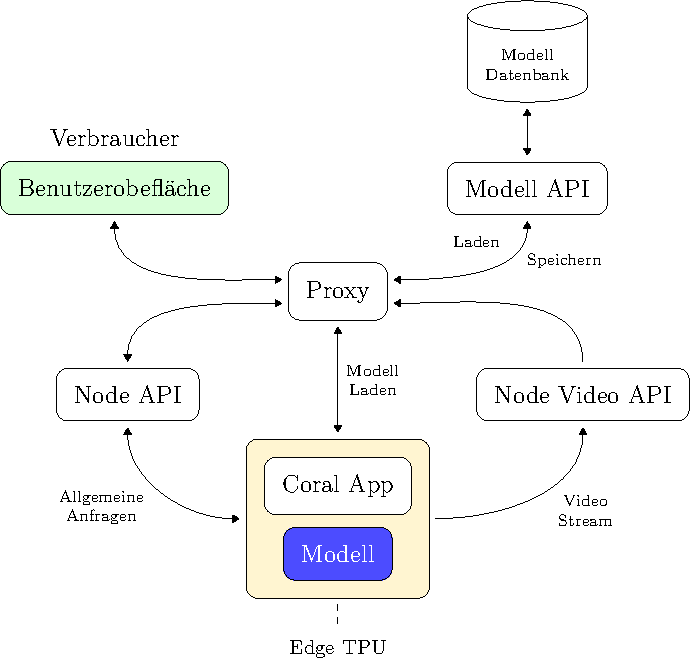
\includegraphics[width=\wLG]{app/app-architecture.pdf}
  \caption{Die Architektur der Anwendung: Ein Modell, das als Dienst
  bereitgestellt wird und verschiedene Services, die mit diesem kommunizieren}
  \label{fig:app-architecture}
\end{figure}

\noindent
Jedes Objekt mit einer Pfeilspitze spiegelt einen Service wieder, insgesamt sind
es sieben Stück. Ein Service ist eine unabhängige, wenn möglich kleine und
unkomplizierte Anwendung, welche nicht mehr als eine Aufgabe übernimmt.
Um die Verwaltung dieser Services zu erleichtern, wird Docker eingesetzt.
Jeder Dienst kann so isoliert in seinem eigenen Docker-Container ausgeführt
und über Docker-Netzwerke verbunden werden.\\[8pt]
Docker ist eine Freie Software, welche auf Linux, Windows und macOS
läuft. Sie erstellt und verwaltet Container
und kann diese sogar orchestrieren.
Docker, Inc., gegründet in 2008 (ursprünglich \textit{dotCloud} und später unter
dem Spitznamen \enquote{Docker}), ist das Unternehmen,
welche die Software entwickelt hat \parencite{onlide:docker-inc}.
Das Wort \enquote{Docker} kommt aus dem Englischen
und bedeutet \textit{\underline{dock} work\underline{er}} --
eine Person im Hafen die Schiffe be- und entlädt.
Es ermöglicht das einfache Teilen von Software
durch Docker-Images (einschließlich aller Abhängigkeiten
und in der Regel geeigneter Standardkonfiguration) und kann
diese mithilfe der Docker-Engine ausführen.
Wird ein Image ausgeführt, erstellt die Engine einen Docker-Container,
mit dem die Anwendung gut isoliert vom restlichen System gestartet wird.
Es ist ähnlich wie eine virtuelle Maschine,
nur viel schneller und schlanker, 
da der Container direkt auf dem Kernel des Hostbetriebssystems aufsetzt
\parencite[11-14]{book:docker-dd} \parencite[672]{book:hands-on-ml}.\\[8pt]
Docker eignet sich somit gut, um eine Anwendung mit der in dieser Arbeit beschriebenen
Zielsetzung zu entwickeln, die jeder herunterladen und mit ein paar Befehlen
auf dem eigenen System ausführen kann. Der Quelltext zur Anwendung
sowie die bisherigen Programme und nicht immer vollständig gezeigten
Ausschnitte, um den Großteil der Abbildungen zu erzeugen,
befinden such auf dem GitHub-Profil des Autors.
Die Docker-Images der in \autoref{fig:app-architecture} zu sehenden
Services sind über Docker Hub verfügbar.
Docker Hub ist eine Plattform zum Teilen von Docker-Images und das als Standard
eingestellte Image-Register einer neuen Installation der Docker Software.
Ein Image-Register enthält ein oder mehrere Image-Repositorys
und diese enthalten wiederum ein oder mehrere Images.
Die folgenden Punkte fassen die wichtigsten Links zusammen:
\begin{itemize}
  \item Der Quelltext zur Anwendung auf GibHub
        (\url{https://github.com/JensDll/coral-ml}).
  \item Die bisherigen Programme und Ausschnitte zum Erstellen der Abbildungen
        (\url{https://github.com/JensDll/bachelorarbeit-notebooks}).
  \item Die Docker-Images der Services auf Docker Hub
        (\href{https://hub.docker.com/repository/docker/jensdll/coral-ml}
        {https://hub.docker.com/reposito\allowbreak ry/docker/jensdll/coral-ml}).
\end{itemize}

\section{Herunterladen und Verbinden der Dienste}
Um ein Image von Docker Hub herunterzuladen, wird
der \pythoninline{docker pull} Befehl verwendet.
Für offizielle Image-Repositorys, die sich
auf der obersten Ebene des Docker Hub Namensraums befinden,
nimmt dieser Befehl die folgende Form an:
\begin{consolecode}
$ docker pull <repository>:<tag>
\end{consolecode}
Es wird das Repository zusammen mit dem gewünschten Image
in der Form eines Tags angegeben.
Offizielle Repositorys sind ein Prinzip von Docker Hub.
Hier befinden sich von Docker Inc. ausgewählte
Images, die speziell geprüft, getestet,
gut dokumentiert und sicher sein sollten.
Die meisten populären und etablierten Anwendungen
und Betriebssysteme haben ihre eigenen
offiziellen Repositorys auf Docker Hub.
Das Abrufen von Images aus inoffiziellen Repositorys
ist im Wesentlichen dasselbe, hierfür
muss dem Repository-Namen
lediglich den Docker Hub Benutzernamen oder die Organisation
vorangestellt werden.
Der folgende Befehl lädt zum Beispiel das neuste
Benutzeroberflächen-Image aus dem \consoleinline{coral-ml}
Repository herunter, das der Person gehört, deren Docker Hub Kontoname
\consoleinline{jensdll} ist:
